\chapter{Результаты экспериментов}
\label{ch:experiments}

Для проведения экспериментов использовались датасет Market-1501, разметка семантических атрибутов Market-1501\_Attribute, а также решение задачи pose estimation с помощью HRNet. В качестве архитектуры визуального энкодера CLIP исползьовалась ResNet-50. Каждый вариант из предложенных модификаций был протестирован с различными значениями гиперпараметров, таких как коэффициент сглаживания в label smoothing, а также количество эпох обучения на второй стадии. Остальные гиперпараметры были зафиксированы на тех же значениях, что и в работа CLIP-ReID. Наилучшими значениями весов лосс-функций также оказались те, что изначально использовались в CLIP-ReID. При этом количество эпох до сходимости модели в некоторых вариантах требовалось большим, чем оригинально. Репозиторий с кодом, использованным для проведения экспериментов, доступен по ссылке: \href{https://github.com/Dentikka/CLIP-ReID}{https://github.com/Dentikka/CLIP-ReID}. 

\section{Сравнение качества методов}

В \hyperref[tab:exp_results]{Таблице \ref*{tab:exp_results}} приведены результаты экспериментов. Полужирным шрифтом обозначен метод с наилучшим качеством - им является исходный метод CLIP-ReID.

Так, в первую очередь было замерено качество базовых методов - CLIP и CLIP-ReID. Также была проверена гипотеза о том, что двухстадийный подход CLIP-ReID может дать дальнейшее улучшение качества при повторении всего процесса обучения еще одну итерацию, благодаря установлению лучшего соответствия между инфорацией разных типов. 

Далее были проведены эксперименты по использованию семантических атрибутов. Так, в одном из экспериментов они использовались для формирования текстовых описаний. В двух других вариантах проверялась возможность применения label smoothing с коэффициентом сглаживания $\lambda = 0.5$, а также модификации метрической лосс-функции умножением на маску соответствия атрибутов. Как видно из таблицы, добавление такого типа сглаживания оказалось излишним и привело к расхождению обучения модели.

Также была проведена серия экспериментов по регуляризации визуального представления на основе информации о позе объекта с помощью конкатенации визуального эмбеддинга с обучаемым эмбеддингом разметки ключевых точек перед проекцией в общее метрическое пространство. 

В одном из вариантов для установления равенства вкладов эбмеддингов изображений и ключевых точек в итоговое представление было добавлено проецирование на единичную сферу, то есть нормировка. В другом варианте, также с целью выравнивания масштаба, производилась номрализация каджого из двух эмбеддингов с помщоью операции, аналогичной батч-нормализации, но не отдельно по каждой компоненте вектора, а нормировакой на одно число $-$ среднюю норму этого вектора. Таким образом построенные эмбеддинги изображения и ключевых точек имели одинаковый порядок масштаба и при этом были распределены более равномерно, а не только на единичной сфере.

Наконец, был рассмотрен вариант с регуляризацией не обучаемым эмбеддингом, а извлекаемым из предобученной модели pose estimation $-$ HRNet, также с применением нормализации. Данная стратегия использовалась только на этапе обучения; на этапе инференса же использовались только визуальные эмбеддинги.

Как следует из \hyperref[tab:exp_results]{Таблицы \ref*{tab:exp_results}}, ни одна из предложенных модификаций не дает улучшения качества по сравнению с исходным методом CLIP-ReID. При этом некоторые методы, основанные на регуляризации, требуют большего числа итераций оптимизации для достижения своего наилучшего результата.

\begin{table}[]
	\centering
	\caption{Сравнение результатов экспериментов}
	\begin{tabular}{|l|l|l|l|l|}
		\hline
		\multicolumn{1}{|l|}{Тип метода} & \multicolumn{1}{l|}{Эксперимент} & \multicolumn{1}{l|}{\#эпох} & 
		\multicolumn{1}{l|}{mAP} & \multicolumn{1}{l|}{CMC@1} \\ \hline
		
		\multirow{3}{*}{\makecell[c]{CLIP-ReID}} & \begin{tabular}[c]{@{}l@{}} Настройка визуальной модели\\ CLIP без первой стадии\end{tabular} & 120 & 88,1 & 94,7 \\ \cline{2-5}
		
		& \begin{tabular}[c]{@{}l@{}} CLIP-ReID с обеими стадиями \end{tabular} & 120 & \textbf{89,8} & \textbf{95,7} \\ \cline{2-5}
		
		& \begin{tabular}[c]{@{}l@{}} Повторение процесса обучения \\ CLIP-ReID 2 раза \end{tabular} & 120 & 89,7 & 95,4 \\ \hline

		\multirow{6}{*}{\makecell[c]{Модификации}} & \begin{tabular}[c]{@{}l@{}} Промпты по атрибутам \\ вместо первой стадии \end{tabular} & 120 & 85,5 & 94,2 \\ \cline{2-5}
		
		& \begin{tabular}[c]{@{}l@{}} Label smoothing по атрибутам \\ на первой стадии \end{tabular} & 120 & 88,9 & 95,6 \\ \cline{2-5}
		
		& \begin{tabular}[c]{@{}l@{}} Label smoothing по атрибутам \\ на обеих стадиях \end{tabular} & 120 & 16,7 & 29,8 \\ \cline{2-5}
		
		& \begin{tabular}[c]{@{}l@{}} Регуляризация эмбеддингом \\ ключевых точек, \\ без нормализации \end{tabular} & 120 & 97,5 & 84,3 \\ \cline{2-5}
		
		& \begin{tabular}[c]{@{}l@{}} Регуляризация эмбеддингом \\ ключевых точек, \\ нормировка \end{tabular} & 360 & 88,1 & 94,9 \\ \cline{2-5}
		
		& \begin{tabular}[c]{@{}l@{}} Регуляризация эмбеддингом \\ ключевых точек, \\ нормализация средней \\ нормой вектора \end{tabular} & 480 & 88,9 & 95,3 \\ \cline{2-5}
		
		& \begin{tabular}[c]{@{}l@{}} Регуляризация эмбеддингом \\ HRNet, нормализация \\ средней нормой вектора \end{tabular} & 480 & 88,1 & 95,1 \\ \hline
	\end{tabular}
	\label{tab:exp_results}
\end{table}


\section{Анализ обученных моделей}

В экспериментах с применением эмбеддинга ключевых точек в качестве регуляризатора для эмбеддинга изображения возможен анализ весов слоя проекции из их пространства в общее пространство, где происходит сопоставление с текстовым эмбеддингом. В частности, при наличии нормализации оба эмбеддинга имеют одинаковый масштаб. Соответственно, возникает возможность сравнить масштаб весов, с которыми они подаются в линейный проектор. 

На \hyperref[fig:proj_weights]{Рисунке \ref*{fig:proj_weights}} приведены гистограммы распределения весов проектора отдельно для компонент эмбеддинга изображения и для ключевых точек. Видно, что в случае обучаемого эмбеддинга (\hyperref[fig:proj_weights_learn]{Рисунок \ref*{fig:proj_weights_learn}}) соответствующие веса концентрируются ближе к нулю по сравнению с компонентами визуального эмбеддинга. При использовании предобученного эмбеддинга HRNet (\hyperref[fig:proj_weights_hrnet]{Рисунок \ref*{fig:proj_weights_hrnet}}) наблюдается та же тенденция, но менее ярко выраженная.

Таким образом, в результате оптимизации модели те ее ветви, которые отвечает за обработку предоставленной дополнительной информации, вносят лишь минимальный вклад в ее работу. Наиболее ярко эта закономерность обнаруживается при построении полностью обучаемого энкодера ключевых точек.

С другой стороны, результаты экспериментов говорят о том, что данная дополнительная ветвь вносит помехи в работу основной модели. В случае, когда данная ветвь является обучаемой, ее вклад минимизируется при оптимизации модели. В случае же работы с фиксированными дополнительными эмбеддингами наблюдается существенный вклад в итоговое представления, однако это сказывается негативным образом на качестве работы модели, которое оказывается хуже, чем в случае с обучаемыми эмбеддингами.

\begin{figure}[ht]
	\centering
	\begin{subfigure}[b]{0.45\textwidth}
		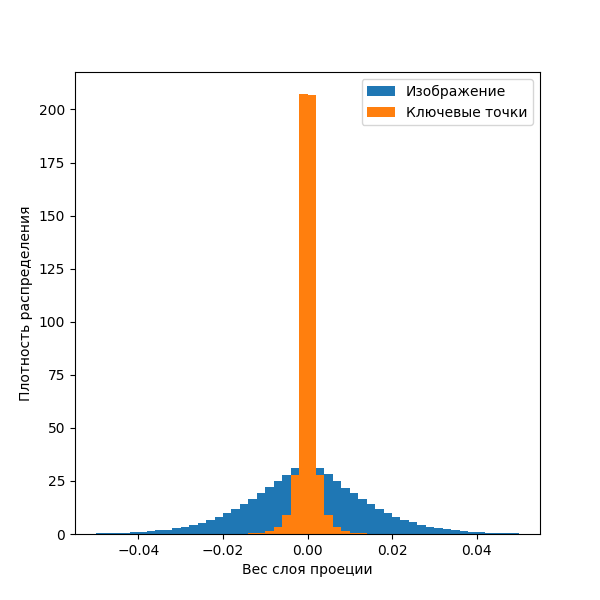
\includegraphics{images/results/analyze_model/concat_normalize.png}
		\caption{Обучаемый эмбеддинг}
		\label{fig:proj_weights_learn}
	\end{subfigure}
	%	\hfill
	\begin{subfigure}[b]{0.45\textwidth}
		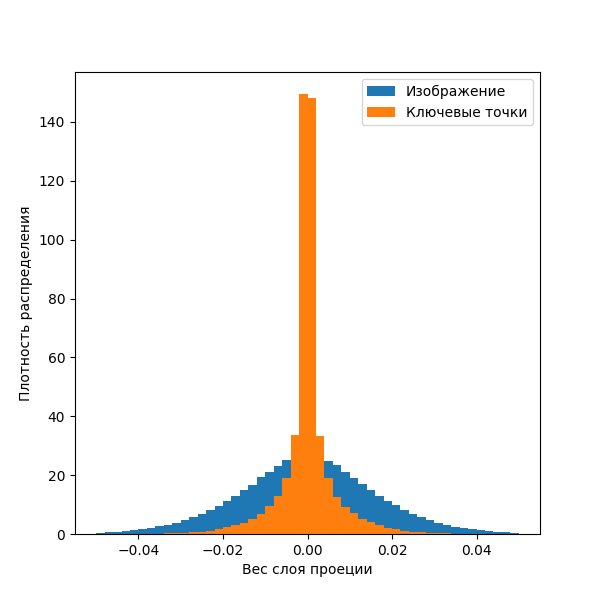
\includegraphics{images/results/analyze_model/concat_hrnet_normalize.png}
		\caption{Эмбеддинг HRNet}
		\label{fig:proj_weights_hrnet}
	\end{subfigure}
	\caption{Распределение весов слоя проекции в общее метрическое пространство. Синим цветом - компоненты эмбеддинга изображения, оранжевым - эмбеддинга ключевых точек.}
	\label{fig:proj_weights}
\end{figure}




